\documentclass{LTHtwocol} % Use this when you work on your report.
% \documentclass[final]{LTHtwocol} % Use this for the final version.
                                   % It will remove page numbers and
                                   % markers for overfull boxes.
                                   % There really shouldn't be any of those anyway.

\usepackage[utf8]{inputenc}
\usepackage{graphicx,xcolor}
\usepackage{hyperref} 
\usepackage{multirow}
\hypersetup{
  colorlinks,
  allcolors={blue!40!black},
}

\usepackage{kantlipsum} % Only for the dummy text. Remove for your own report.

\addbibresource{bibliography.bib}

% Document begins here
\begin{document}
\begin{frontmatter}
\title{Balancing the Furuta Pendulum using different Reinforcement Learning and Control Methods} % Title of the project.
                      % Note that all reports are in English,
                      %so that our international students can read them.

\author[hashim]{Hashim Ismail}
\author[jingmo]{Jingmo Bai}
\author[julien]{Julien Moreau}
\author[yuyang]{Yuyang Jin}

\email[hashim]{ha7172is-s@student.lu.se}
\email[jingmo]{ji8255ba-s@student.lu.se}
\email[julien]{ju6623mo-s@student.lu.se}
\email[yuyang]{yu4020ji-s@student.lu.se}

\advisor[johan]{Johan Grönqvist}
\email[johan]{johan.gronqvist@control.lth.se }
% There is also \affiliation, with the same pattern as \email

\begin{abstract}
    The goal of this project is to balance the Furuta Pendulum upward using various learning techniques and to compare the results. In this work, we explore different settings ranging from a complete black-box to grey and white-box. Balancing the pendulum can be achieved using classical control theory but this requires knowing the parameters of the system and/or splitting the controller to handle non-linear behavior. Black box Reinforcement Learning models such as TD3 learn only from trial and error on the system. Greyer box models can benefit from an automatic control perspective to improve robustness. Finally, white box models have the most potential but can be tricky to transfer into the real world. To speed up the learning process, we use a simulated model of the pendulum as a training environment before deploying the models to the real pendulum.
\end{abstract}

\end{frontmatter}

% Stick to the proposed structure below. Add \subsections{} as appropriate.
% This file compiles on the Automatic Control Department system by typing the
% following into the terminal (while in the directory of the file, and with all
% other files belonging to the template untouched):
% > pdflatex template        
% > biber template
% The first line compiles the .tex file. The second line generates the
% bibliography. Once this is done, you may need to run the first line 1-2
% additional times, for the system to get all cross references right in the
% produced pdf output.

\section{Introduction}
% Here you introduce the project. What is the background? What project do you aim at solve? References to prior work? If the project makes a positive or negative environmental, or other solitary, impact, describe it here. Are there any ethical considerations? You might want to reference relevant literature, e.g. \cite{openclosed2, Hellerstein2004, Yun2015}. A general \LaTeX\ guide is available at \cite{latexwiki}. 

\subsection{Furuta Pendulum}
The Furuta Pendulum is a type of inverted pendulum, the control of which is a classic control theory problem in robotics and engineering. It consists of a pendulum arm that can rotate in the vertical plane, a joint section which connects the arm and the base, and a motorized rotary base that can rotate the pendulum base in the horizontal plane. Figure~\ref{fig:furutapendulum} shows the construction of a typical furuta pendulum.

The unique feature of the Furuta Pendulum is that the rotary base is perpendicular to the pendulum arm, allowing for a wider range of motion and more complex control problems than other inverted pendulums. The pendulum's movement is affected by the rotary base's motion and vice versa, making the system highly nonlinear and challenging to control.

The Furuta Pendulum has become a popular platform for research in control theory and robotics because it presents a challenging control problem that requires sophisticated control algorithms to stabilize the pendulum in the inverted position. Its applications include studying human motor control, developing advanced control algorithms for robotics, and testing control systems in spacecrafts and other unstable platforms.

\begin{figure}[b]
	\centering
	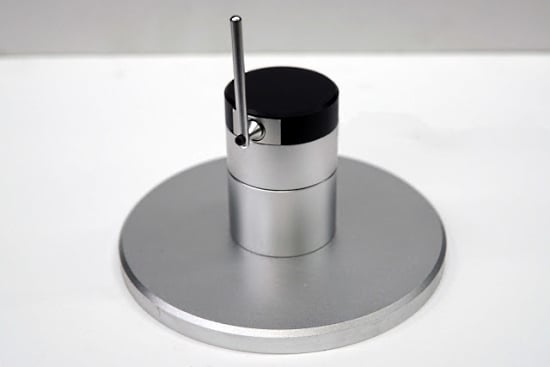
\includegraphics[width=0.7\columnwidth]{pic/furutapendulum.jpg}
	\caption{Picture of the Furuta Pendulum}
	\label{fig:furutapendulum} % Should be placed after the caption!
\end{figure}

\subsection{Reinforcement Learning}
Reinforcement learning (RL) is a type of machine learning in which an agent learns to make decisions through trial and error interactions with an environment. The goal of RL is to maximize a reward signal by selecting actions that lead to positive outcomes while avoiding actions that lead to negative outcomes.

RL is different from other machine learning approaches because it focuses on how agents can learn to make sequential decisions in dynamic environments. The agent learns by receiving feedback in the form of a reward signal, which indicates the success or failure of its actions. Through repeated interactions with the environment, the agent learns to associate certain actions with positive outcomes and others with negative outcomes, allowing it to make more informed decisions in the future.

RL has found applications in a wide range of fields, including robotics, game development, finance, and healthcare. RL algorithms have been used to train robots to perform complex tasks, such as grasping and manipulating objects, and to develop intelligent agents that can play complex games, such as chess and Go, at a superhuman level.

\section{Modeling}

The abstract model of the pendulum is shown in Figure~\ref{fig:abstractmodel}. The integration model derived in Magnus Gäfvert's report \cite{2efe5c5060d9449683ba4bc412e9acef} is used in this project, which is presented below \eqref{eq:integrationmodel}.

\begin{figure}[b]
	\centering
	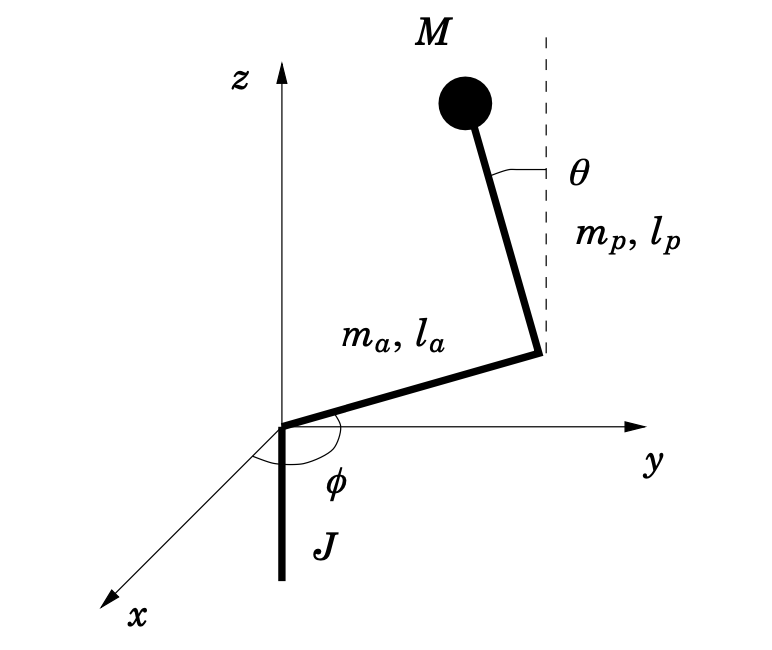
\includegraphics[width=0.7\columnwidth]{pic/absmod.png}
	\caption{Abstract model of the Furuta Pendulum}
	\label{fig:abstractmodel} % Should be placed after the caption!
\end{figure}
\begin{table*}
\begin{equation}
\begin{aligned}
    \frac{d}{dt}\phi & = \dot{\phi}\\
    \frac{d}{dt}\dot{\phi} & = \frac{1}{\alpha \beta - \gamma^{2}+(\beta^{2} + \gamma^{2}) \sin^{2} \theta}\{\beta \gamma (\sin^{2} \theta - 1)\sin \theta \dot{\phi}^{2}
    -2 \beta^{2} \cos \theta \sin \theta \dot{\phi} \dot{\theta} + \beta \gamma \sin \theta \dot{\theta}^{2} - \gamma \delta \cos{\theta} \sin{\theta}
    + \beta \tau_\phi - \gamma \cos{\theta \tau_\theta}\} \\
    \frac{d}{dt}\theta & = \dot{\theta} \\
    \frac{d}{dt}\dot{\theta} & = \frac{1}{\alpha \beta - \gamma^{2}+(\beta^{2} + \gamma^{2}) \sin^{2} \theta}\{\beta (\alpha + \beta \sin^{2}\theta) \cos{\theta}
    \dot{\phi}^{2} + 2 \beta \gamma (1 - \sin^{2}\theta) \sin{\theta} \dot{\phi} \dot{\theta} - \gamma^{2} \cos{\theta} \sin{\theta} \dot{\theta}^2 + \delta (\alpha + \beta \sin^{2} \theta) \sin{\theta} \\
    & - \gamma \cos{\theta \tau_\theta} + (\alpha + \beta \sin^{2} \theta)\tau_\theta \}
\end{aligned}
\label{eq:integrationmodel}
\end{equation}
\vspace{3pt}
\hline
\end{table*}
In the equations of motion $\theta$ and $\phi$ represent the arm angle and the base angle respectively and the parameters $\alpha$, $\beta$, $\gamma$ and $\delta$ have the following meanings:
\begin{equation}
\begin{aligned}
    \alpha &\triangleq J + (M + \frac{1}{3} m_a + m_p)l^2_a \\
    \beta &\triangleq (M + \frac{1}{3} m_p)l^2_p \\
    \gamma &\triangleq (M +\frac{1}{2} m_p)l_a l_p \\
    \delta &\triangleq (M + \frac{1}{2} m_p)gl_p 
\end{aligned}
\end{equation}
where all the involved parameters can be measured from a real pendulum\cite{2efe5c5060d9449683ba4bc412e9acef}, see Table~\ref{tab:pendulumparameters} and Table~\ref{tab:modelparameters}.

\begin{table}[t]
	\centering
	\caption{Real pendulum parameters}
	\label{tab:pendulumparameters}
	\begin{tabular}{cccccc} % (l)eft, (r)ight and (c)enter indentation
		\toprule
        $J$[kg$\cdot m^2$]     & $l_p$[m]  & $m_a$[kg] & $l_a$[m] & $M$[kg]     & $m_p$[kg]         \\ 
        \midrule 
        9.72e-5 & 0.413 & 0.072 & 0.25 & 0.00 & 7.75e-3  \\
	\end{tabular}
\end{table}

\begin{table}[t]
	\centering
	\caption{Model parameters}
	\label{tab:modelparameters}
	\begin{tabular}{cccc} % (l)eft, (r)ight and (c)enter indentation
		\toprule
        $\alpha$[kg$\cdot m^2$] & $\beta$[kg$\cdot m^2$] & $\gamma$[kg$\cdot m^2$] & $\delta$[kg$\cdot m^2/s^2$]      \\ 
        \midrule 
        0.0033472 & 0.0038852 & 0.024879 & 0.097625  \\
	\end{tabular}
\end{table}

Introduce the state variable 
$$ x \triangleq \begin{pmatrix}
\phi \\ \dot{\phi} \\ \theta \\ \dot{\theta}
\end{pmatrix}$$
and linearize the model at the equilibrium point $x_0 = (\phi_0, \dot{\phi}_0, \theta_0, \dot{\theta}_0)$ with $\delta x \triangleq x- x_0$.
\begin{equation}
    \frac{d(\delta x)}{dt} = A\delta x + B\tau
\label{eq:linequ}
\end{equation}
For the upwards position $x_0 = (0,0,0,0)$ we have $$A = \begin{pmatrix}
0 & 1 & 0 & 0 \\
0 & 0 & -\frac{\delta\gamma}{\alpha\beta - \gamma^2} & 0 \\
0 & 0 & 0 & 1 \\
0 & 0 & \frac{\alpha\delta}{\alpha\beta - \gamma^2} & 0 
\end{pmatrix}, B = \begin{pmatrix}
0 & 0 \\
\frac{\beta}{\alpha\beta - \gamma^2} & -\frac{\gamma}{\alpha\beta - \gamma^2} \\
0 & 0 \\
-\frac{\gamma}{\alpha\beta - \gamma^2} & -\frac{\alpha}{\alpha\beta - \gamma^2}
\end{pmatrix}$$


\section{Simulation Environment}

Once the equations and parameters are estimated, we can use a differential equation solver to compute the motion of the pendulum. In our case, we first tried solving the equation system with the Julia \textit{DifferentialEquation.jl} package\cite{rackauckas2017differentialequations}. We later found out that a ready implementation was available with the \textit{FurutaPendulums.jl} package and ended up relying on this code instead. The principle is the same for both approaches: given a state $x_t = [\phi,\dot\phi,\theta,\dot\theta]$, estimate the state $x_{t+dt}$ by evaluating the derivative $\dot x = f(x,t)$ around t.

A popular method is to use a Runge Kutta variant such as the 3/8 variant:
\begin{align*}
k_1 &= dt f(t, x_t)\\
k_2 &= dt f(t + dt / 3, x_t + k_1 / 3 )\\
k_3 &= dt f(t + 2 dt / 3, x_t - k_1 / 3 + k_2 )\\
k_4 &= dt f(t + dt, x_t + k_1 - k_2 + k_3 )\\
x_{t+1} &= x_t + 1/8 ( k_1 + 3 k_2 + 3 k_3 + k_4 )
\end{align*}

More precise methods rely on complex schemes and use adaptative time steps but RK3/8 to return satisfying results, see Figure \ref{fig:sim} for a comparison with the real pendulum. The dangers of using an improper simulation environment is that models will have a harder time when applied in the real world. This is especially important for white-box models that expect an exact representation of the environment. In the case of TD3, the training can be resumed in the real environment to adapt to the differences.

\begin{figure}
    \centering
    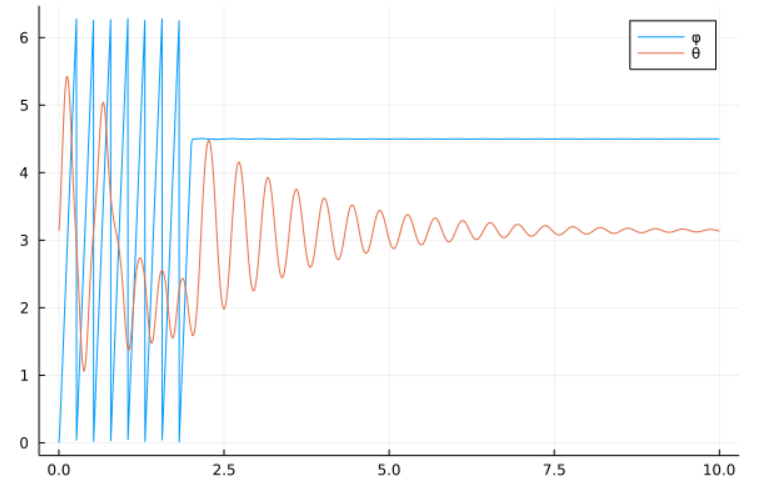
\includegraphics[width=0.7\columnwidth]{pic/real.png}
    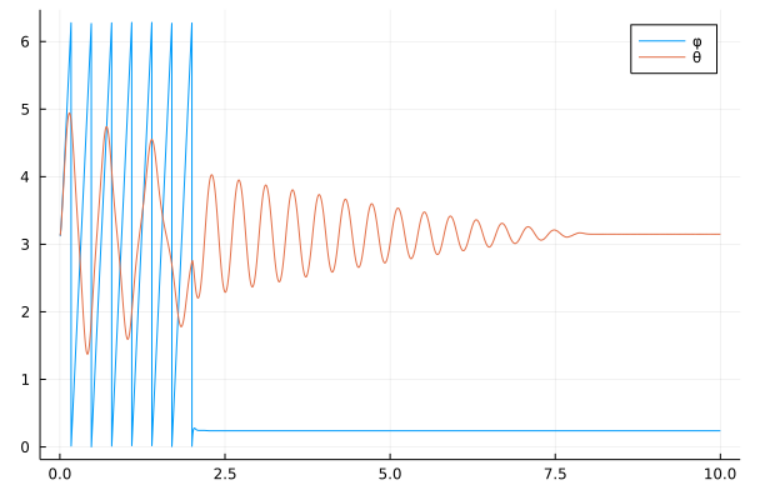
\includegraphics[width=0.7\columnwidth]{pic/sim.png}
    \caption{Pendulum motion from the real pendulum (top) and the simulation (bottom). The angles were recorded after using a simple control signal: u=2.5V for 2 seconds then u=0. The curves show slight differences but the behavior seems to be close enough for our purposes.}
    \label{fig:sim}
\end{figure}

\section{Model-free TD3}

\subsection{Algorithm}
The algorithm we use is TD3(Twin Delayed Deep Deterministic Policy Gradient)\cite{fujimoto2018addressing}, which is an advanced and improved version of DDPG(Deep Deterministic Policy Gradient)\cite{lillicrap2015continuous}. 

DDPG is an algorithm that learns a Q-function and a policy at the same time. The Q-function is learnt from off-policy data and the Bellman equation, and the policy is learnt from the Q-function.

For the Q-learning part, first, the optimal action-value function $Q^\ast(s,a)$ is given by the Bellman equation
\begin{equation}
    Q^\ast(s,a)= \displaystyle \mathop{\mathbb{E}}_{s'\sim P} [r(s,a)+\gamma \max_{a'}Q^\ast(s',a')]
\end{equation}

We have a neural network $Q_\phi(s,a)$ with parameters $\phi$, a set $D$ of transitions $(s,a,r,s',d)$(where d indicates whether state $s'$is terminal). And we try to minimize a mean-squared Bellman error(MSBE) loss function.
\begin{equation}
\begin{aligned}
L(\phi,D)&=\displaystyle \mathop{\mathbb{E}}_{(s,a,r,s',d)\sim D} \bigg[\bigg(Q_\phi(s,a)\\&-
\Big(r+\gamma(1-d)\max_
{a'} Q_\phi(s',a')\Big)\bigg)^2\bigg]
\end{aligned}
\end{equation}
In the equation above, the term
\[
r+\gamma(1-d)\max_{a'} Q_\phi(s',a')
\]
is called the target, the problem is it depends on the same parameters $\phi$ we are trying to train. The solution is to use a set of parameters which are close to $\phi$, but with a time delay, which is a second network called the target network. In DDPG, the target network is updated once per the main network update.

For the policy learning part, we want to learn a deterministic policy $\mu_\theta(s)$ which gives the action that maximizes $Q_\phi(s,a)$. Because the action space is continuous and we assume the Q-function is differentiable with respect to action, we can perform gradient ascent with respect to policy parameters to solve
\[
\max_\theta \displaystyle \mathop{\mathbb{E}}_{s'\sim D}[Q_\phi(s,\mu_\theta(s))]
\]

Finally, DDPG is performed by minimizing the following MSBE with stochastic gradient descent:
\begin{equation}
\begin{aligned}
L(\phi,D)&=\displaystyle \mathop{\mathbb{E}}_{(s,a,r,s',d)\sim D} \bigg[\bigg(Q_\phi(s,a)\\&-\Big(r+\gamma(1-d) Q_{\phi_{targ}}(s',\mu_{\theta_{targ}}(s'))\Big)\bigg)^2\bigg]
\end{aligned}
\end{equation}

Sometimes, there could be problems when tuning the hyperparameters using DDPG. For example, a common failure mode is that the learned Q-function begins to dramatically overestimate Q-values because it exploits the errors in the Q-function. Twin Delayed DDPG(TD3) is an algorithm that can deal with this issue.

There are 3 main improvements in TD3 compared to DDPG.

First, TD3 learns two Q-functions instead of one and uses the smaller of the two Q-values to form the targets in the Bellman error loss function. It helps to prevent overestimation in the Q-function. The target is given by:
\begin{equation}
    y(r,s',d)= r+\gamma(1-d)\min_{i=1,2} Q_{\phi_{i,targ}}(s',a'(s'))
\end{equation}

Then both Q-functions are learned by minimizing the MSBE loss with gradient descent:
\begin{equation}
\begin{aligned}
L(\phi,D)&=\displaystyle \mathop{\mathbb{E}}_{(s,a,r,s',d)\sim D} \bigg[\Big(Q_{\phi}(s,a)-y(r,s',d)\Big)^2\bigg]
\end{aligned}
\end{equation}

Second, TD3 updates the policy and target networks less frequently than the Q-function to dampen the volatility that normally arises in DDPG. Usually, we do one policy update for every two Q-function updates. The policy is learned by maximizing $Q_{\phi_1}$:
\[
\max_\theta \displaystyle \mathop{\mathbb{E}}_{s\sim D}[Q_{\phi_1}(s,\mu_\theta(s))]
\]

Third, TD3 adds clipped noise to each dimension of the target action, to make it harder for the policy to exploit Q-function errors, for example, a sharp peak, by smoothing out Q along changes in action. The target actions are thus:
\begin{equation}
    a'(s')=clip(\mu_{\theta_{targ}}(s')+clip(\epsilon,-c,c),a_{Low},a_{High})
\end{equation}
\[
\enspace \epsilon \sim \mathcal{N}(0,\sigma)
\]
\subsection{Configurations}
The reward function we use in TD3 is based on the potential energy at the upwards position minus the total energy currently.
\begin{equation}
    Reward=-|\frac{1}{2}m_p g l_p (1-\cos\theta) - \frac{1}{6} m_p l_p^2 \dot{\theta}^2|
\end{equation}
We want the total energy of the pendulum to be equal to the potential energy at the upwards position with 0 kinetic energy, which can keep the pendulum balanced. The larger the difference, the less the reward value. The goal is to reach a reward of 0.

The discount factor $\gamma$ is set as 0.99. The polyak averaging parameter $\rho$ for updating the target network is set as 0.99. 
For the neural network of the actor and the critic model, after the input layer, we have 30 nodes as the second layer with Relu as the activation function. Then, another 30 nodes are connected as the third layer with the same Relu activation function. At last, a single node is the output layer with Tanh as the activation function. The batch size we use is 64. At the 1000 steps in the beginning, we start with a random policy. After that, we have one policy update for every two Q-function updates. We add a noise of 0.1 to the target action.

\subsection{Training results}
It takes around 4 minutes to train 400 episodes in the simulation environment using JuliaReinforcementLearning\cite{Tian2020Reinforcement}. The model can swing up and stabilize the pendulum within one second. It works fairly well in the simulation environment, given that we only train it for 4 minutes. 

When applying the model to the real pendulum, it can work to some extent, but not as stable as in the simulation environment. Given that the model is trained for only 4 minutes and 400 episodes, we think this approach is a promising one and could perform better after more training time.

\section{PD control with TD3}
The PD model consists of state feedback control. The control signal is the dot product of a gain vector and the measured pendulum state. The task of the TD3 reinforcement learning model this time is to predict suitable gain values for the state.
\begin{figure}[h]
    \centering
    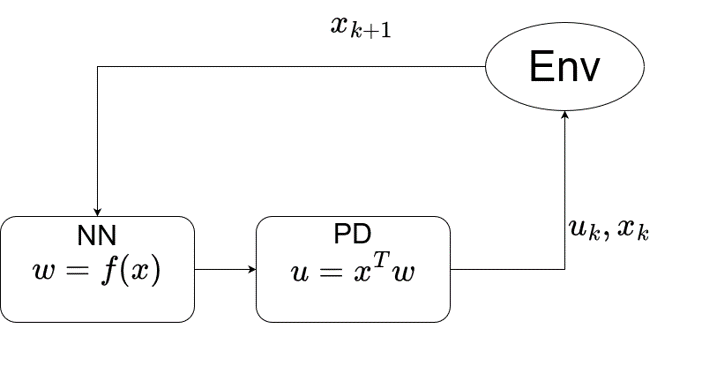
\includegraphics[width=0.7\columnwidth]{pic/PD.png}
    \caption{PD controller with TD3}
    \label{fig:my_label}
\end{figure}
\begin{equation}
    u(t) = - \omega_1 x - \omega_2 \dot x
\end{equation}
$\omega_1$ represents the proportional part of the controller and $\omega_2$ represents the derivative part. This control rule will drive the state to zero which is our desired state. To follow any other reference state $x_r$ that is not zero, we can simply replace $x$ with the error measurement defined by $x_r - x$.
\begin{equation}
    u(t) = \omega_1 (x_r - x) + \omega_2 (\dot x_r - \dot x)
\end{equation}
Solving the pendulum swing up problem using a PD controller is quite hard to do with constant gain parameters because it would require different control behavior at each range of pendulum states. In theory, The pendulum swing up and stabilization process can be split up into multiple stages and a PD controller could be designed for each stage with fixed parameters for each controller to solve the problem. Using the TD3 algorithm we can train an agent to predict suitable parameters at each state without having to split the problem and this will result on a more flexible controller.

\subsection{Configurations}
\textbf{PD design:} The state feedback chosen is simply a vector of the pendulum angles and speeds. Two angles were used for pendulum arm. The base angle was not included to reduce the state space making it easier for the model to converge as it doesn't affect the pendulum arm dynamics. Using $mod2pi$ function, we can keep the arm angle measurement in the range of $0$ to $2 \pi$. Another alternative option is to use the $cos$ and $sin$ of the angle instead.
\begin{equation}
    u = \begin{bmatrix}
        w_{d\phi} \\ w_{mod2pi(\theta)} \\ w_{d\theta}
    \end{bmatrix}
    .- \begin{bmatrix}
        \dot \phi \\ mod2pi(\theta) \\ \dot \theta
    \end{bmatrix}
\end{equation}
\textbf{TD3 design:}
The reward function used is similar to the one we implemented on the black box TD3 implemented in the first experiment with the only difference of added small penalty on the base energy that is only applied if the pendulum is not in the upwards position. This is to produce a more stable behavior and prevent the pendulum from getting high energy in the downwards position.
\[Reward= \]
\begin{equation}
    \begin{cases}
    -|\frac{1}{2}m_p g l_p (1-\cos\theta) - \frac{1}{6} m_p l_p^2 \dot{\theta}^2| \\ \text{if} \,\, cos(\theta)>0.8
    \\ -|\frac{1}{2}m_p g l_p (1-\cos\theta) - \frac{1}{6} m_p l_p^2 \dot{\theta}^2 - \frac{1}{2}J\dot \phi^2 | \\ \text{if} \,\, cos(\theta)<0.8
\end{cases}
\label{reward}
\end{equation}
While the neural networks architecture of the critic networks was not changed from the black box TD3, output of the actor networks were changed to 5 outputs instead of one.

Critic:  $4,30,30,1$

actor: $5,30,30,5$

All the other settings were the same as in the black box experiment.

\subsection{Training Results}
Training the model on the simulation environment for 500 episodes took around 12 minutes to finish. The model was able to swing up the pendulum and stabilize it and showed a promising performance.

Deploying the trained model on the real pendulum, the model managed to swing the pendulum but not keep in the upwards position. This is due to the differences between the simulation and real environment.

By resuming the training on the real environment for an additional 100 episodes on top of the 500 that was done on the simulation, the model was able to swing and stabilize the real pendulum upwards and produced a more stable behavior than the black box model.
Figure (5) below shows how the parameters change over time.
\begin{figure}[h]
    \centering
    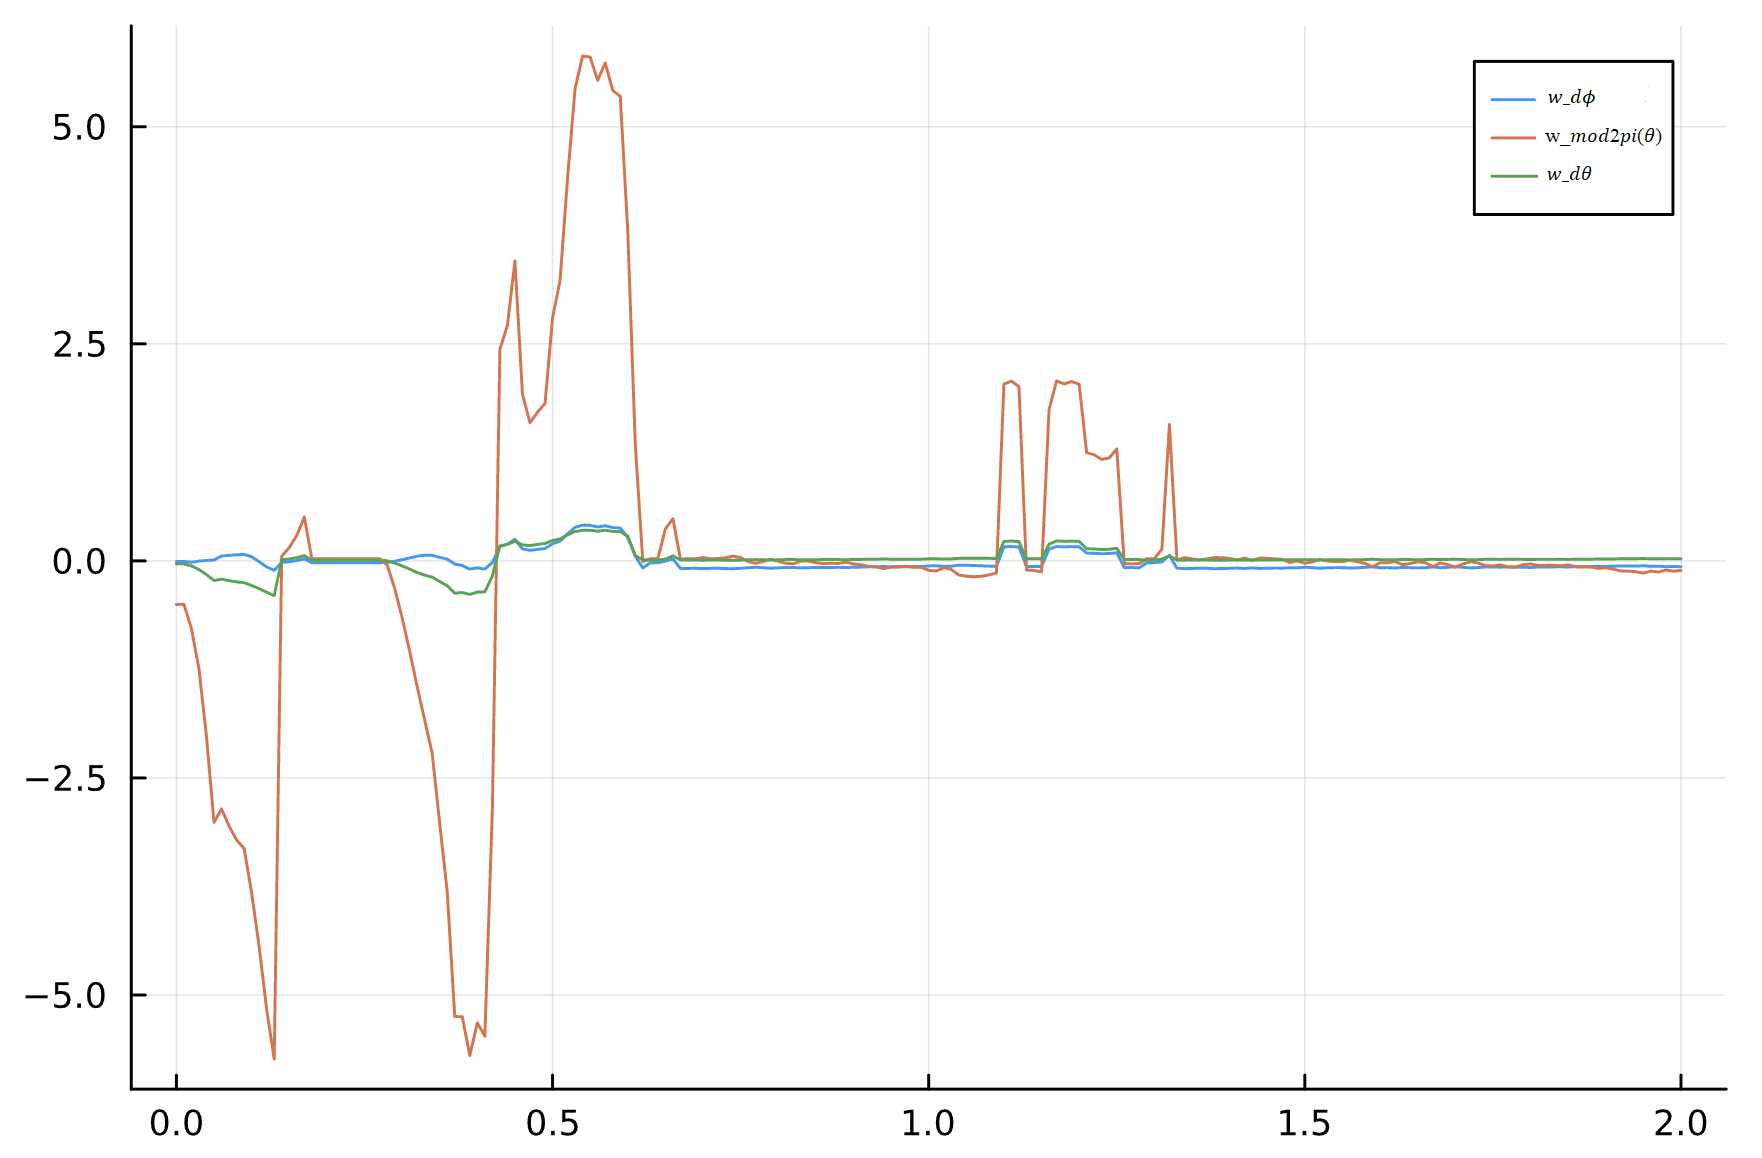
\includegraphics[width=0.7\columnwidth]{pic/pd params.png}
    \caption{TD3 policy output of PD parameters}
    \label{fig:my_label}
\end{figure}

\section{Model Predictive Control}
Model predictive control(MPC) can well handle complex systems, consider constraints, and optimize performance over a finite time horizon, making it applicable to various control tasks. In the project, we designed a non-linear MPC and a linear MPC to handle both the swing-up and balancing problem. It turns out the former method works well for the entire process while the other has some problem in swinging the arm up.

\subsection{Theory}
In MPC, a dynamic model of the system is used to predict the system's future states based on current measurements and control inputs. These predictions are then used to optimize a control action over a finite time horizon, taking into account system constraints and performance objectives. The basic steps involved in MPC are as follows (see also figure~\ref{fig:MPCdiag}):\\
\textbf{Model formulation:} A mathematical model of the system is developed, typically based on physical laws or system identification techniques. The model describes how the system's states and outputs evolve over time.\\
\textbf{Prediction:} Using the model and current measurements, future system states are predicted over a finite time horizon. This is usually done by solving a set of dynamic equations, such as a state-space or differential equation representation.\\
\textbf{Optimization:} An objective function is defined to optimize the control action over the prediction horizon. This objective function includes criteria like tracking setpoints, minimizing error, or energy consumption. Constraints, such as input saturation or process limits, are also considered.\\
\textbf{Control action determination:} The optimization problem is solved to find the optimal control trajectory over the prediction horizon. Typically, numerical optimization techniques like quadratic programming are used.\\
\textbf{Implementation:} The first control action of the optimized trajectory is applied to the system. The process is repeated at each time step, and the control action is continually updated based on new measurements and predictions.

\begin{figure}[t]
	\centering
	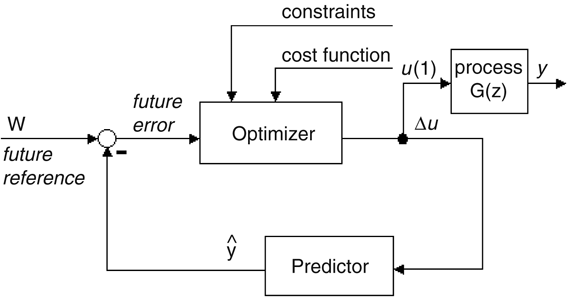
\includegraphics[width=0.9\columnwidth]{pic/MPCdiagram.png}
	\caption{Schematic diagram of MPC}
	\label{fig:MPCdiag} 
\end{figure}

\subsection{Non-linear MPC}
As described above, the model of the furuta system\eqref{eq:integrationmodel} is non-linear. It is natural to implement a non-linear controller in the first place.

We used the dynamics equations\eqref{eq:integrationmodel} as model formulation, set prediction horizon as 10 steps in the future, and choose the simplest objective function $$J = 1 - cos(\theta)$$ which is easy to understand since $\theta$ is 0 when the function is minimized. Note also that constraints on state variables and control signals $$[0.0, -30, 0.0, -30] \leq x \leq [2\pi, 30, 2\pi, 30]$$ $$-5 \leq u \leq 5$$ were added during training to prevent them from exceeding the physical limitations or boundaries.

\subsection{Linear MPC}
Considering the complexity of the dynamics equations may lead to long computation time, we also tried to use linear MPC at the equilibrium point $x_0 = (0,0,0,0)$. Equation \eqref{eq:linequ} was used as model formulation. Other than that, all of the parameter settings were the same as that in non-linear MPC.

\subsection{Training Results}
It takes around 4 minutes to train the non-linear MPC model. This model is able to both swing the arm up and balance it in the simulation environment. The result shows it fell twice in  five seconds of simulation but both swung up in a short time. However, training detail shows that the computation time per iteration varies a lot, most of which are in the range (0.03s, 0.1s), making it impossible to apply on a real pendulum as it exceeds the sampling time(0.01s).

The training time of the linear model is approximately 90 seconds, which is an advantage compared with the non-linear model. However, the pendulum arm could only stay upright for less than one second and would never swing up. It is unsuccessful but also promising because the control signal was actually trying to balance the pendulum arm, only it was always a little lower than the desired value. One possible way to fix this problem is to introduce a coefficient to the determined control action in order that it is not too weak. Considering the limited time, we didn't delve into this problem.

\section{AlphaZero}

AlphaZero was introduced by Silver et al. \cite{10.1038/nature24270} and is an algorithm that learns to play games such as Go and Chess. This assumes that the game environment is known so this approach can be regarded as a white-box controller. Contrary to MPC the system doesn't need more insight into the equations (e.g. the gradients or anything related to optimization). The strategy is only learned via self-play to maximize a user-defined reward.

\subsection{Game Environment}

The algorithm can be applied to any single player game as long as the following assumptions hold:
\begin{itemize}
    \item The game can be decomposed into discrete states and the player have a finite number of possible actions.
    \item We have full information over the state of the game.
    \item Given the current state and action, we can always predict the next state.
\end{itemize} 
We need to fully discretize the state space and the action space. Then, we trust our simulation model to accurately predict the next state.
To take advantage of the tree search, we limit the number of states to the following:
\begin{itemize}
    \item Base speed $\dot\phi$: 100 states in $[-20,20]$ rad.s$^{-1}$.
    \item Arm angle $\theta$: 90 states in $[-\pi,\pi]$.
    \item Arm speed $\dot\theta$: 100 states in $[-50,50]$ rad.s$^{-1}$.
    \item Control action $u$: 3 states -1, 0 and 1V.
    \item Base angle $\phi$: Since it doesn't affect the motion, we can safely ignore this parameter.
\end{itemize}
Note that this discretization scheme is not the best by any mean and could be improved. Similar to the other models, we use a time step of $dt=0.02$ and the same energy reward function. The game ends when the time reaches 5 sec.


One limitation is that the simulated pendulum must always return the same output given a state action pair. This means that the real continuous state has to be "corrected" every time step to match the discretization. Otherwise, the simulation would return different outputs for the same discretized state, thus leading to a "stochastic" game environment.

\subsection{Learning Algorithm}


At the core of AlphaZero is a neural network that takes a state as input and outputs both the  policy $\vec{p}$ vector (probability to take each control action) and the value $v$. To train the network, the Reinforcement Learning algorithm alternates between "self-play" and "learning" phases.


During self-play the agent uses a Monte Carlo Tree Search to play and explore the best policy. Without going into the details of MCTS, the agent expends a tree of possible actions into the future and computes the value of the encountered states with the neural network. The algorithm can then estimate the optimal policy in the given state as a probability vector $\vec{\pi}_t$ (here of length 3). A random move is then sampled based on the probabilities in $\vec{\pi}$. The process is repeated every timestep until the game ends.


In the learning phase, the network is trained on the data $(s_t, \pi_t, r_t)$ from previous games. The loss function is a combination of a negative cross-entropy on the policy and a squared error on the value.
$$l = \sum_t (v(s_t) - r_t)^2 - \vec{\pi}_t \cdot \log(\vec{p}(s_t))$$
Where $r_t$ is the reward at time $t$, $\vec{p}(s_t)$ and $v(s_t)$ are the network's estimate of the policy and value.

Regularly during training, we play a game using the current network and the one updated with the new data. If the cumulated reward of the updated network is greater than the current one, then we replace it.

\subsection{Training Results}

We use a julia package \cite{Laurent2020AlphaZero} to train AlphaZero on 320 episodes using 50 MCTS iterations every time step, this took around 2 hours on a computing server. The agent achieves very good results on the discrete simulation, balancing the pendulum in less than a second. However, this is a very idealized playground and does not reflect reality. When transferred to a continuous simulation, the agent is more shaky but still achieves a quick swing up. However, the MCTS tree search is computer intensive and we have to reduce the tree exploration depth for real-time play.

When confronted to a continuous, real-time simulation, the agent is less stable but shows encouraging behavior. It manages to swing up the pendulum in the simulation in 7 sec but fails to balance it for more than a second. 

One drawback of this approach is that it is not straight forward to introduce noise during training. 

\section{Discussion}
\begin{table*}[]
\centering
\caption{Comparison Table}
\label{tab:comparison}
\begin{tabular}{lccccl}
\vspace{6pt}
\textbf{Model} & \textbf{Episodes} & \textbf{Training time} & \textbf{Swing up (Simulation)} & \textbf{Swing up (Real)} & \textbf{Robustness} \\ \hline \\
\textbf{TD3} & 400 & 4 min & Yes & Yes & Good, swings back up\\
\vspace{6pt}
& & & & &  when pushed \\
\textbf{PD TD3} & 500 & 12 min & Yes & Yes & Very good, holds up \\
\vspace{6pt}
& & & & & when pushed \\
\textbf{MPC} & N/A & N/A & Yes & No & N/A \\ \\
\vspace{6pt}
\textbf{AlphaZero} & 400 & 2 hours & Yes & No & N/A
\vspace{6pt}

\end{tabular}
\end{table*}
\paragraph{Reward functions} One of the challenges we encountered was the algorithms exploiting the reward function. The first idea was to put an absolute error on the arm angle. However, we found that the agent learned to spin the arm really fast, that way it could get to the upwards position every time step then do a complete rotation between each reward evaluation. We then thought about putting an additional penalty on the speed of the arm, but this ended up slowing the learning process. With a penalty on speed, the model just learns to stay still and doesn't explore other positions. Finally, we tried an energy-based cost function, which requires a bit of knowledge about the physics of the pendulum. The results were better but some models still managed to exploit the objective by oscillating very fast in the downwards position. The reward function was thus modified one last time (see Eq \ref{reward}), it is far from perfect but the algorithm didn't manage to exploit it.

\paragraph{Comparison} Both the PD and the black box TD3 models produced great results and managed to stabilize the pendulum in the upwards position. The training time for each was good around 5 to 12 minutes and done within around 400 episodes in the simulation environment. However, the PD model produced a more stable behaviour and the parameters were more interpretable. MPC and AlphaZero did not produce viable controllers for the real pendulum, the amount of time they spend processing at each time step is too high to achieve good performance. This implies that methods such as MPC and AlphaZero are not really suited for very responsive systems that react in a fraction of a second. These algorithms would perform better in bigger scale, slower systems. Another point is that training AlphaZero took a lot more time than black box methods. This is a bit disappointing given that AlphaZero has a head start since it already knows the model.

\paragraph{Future Improvements} Overall we believe that all models have much more room for improvement if more time was spent to fine-tune and adjust their settings. The TD3 black box model could benefit from adjusting the reward function by adding a penalty on the base angle. The PD model could be improved by adding an integral part turning it into a PID controller which will improve stability. The MPC model could be further optimized by scheduling the processing time to run while the environment is executing the solution for the previous time step to make sure an optimal solution is reached before the next time step.

\paragraph{Lessons from the project} We've learnt that it is important to have an accurate simulation of the real object. One reason is that different group members can train and test their models at the same time with a simulation. Moreover, our project involves long hours of training, which may lead to damage to the equipment. During the project, we found that the implementation on a real object could place additional demands.


% Prints cited references
\printbibliography


\end{document}


